\subsection{Overview}
The architecture of the system is composed of two main components: the \ac{eMSP} and the \ac{CPMS}.

The \ac{eMSP} follows the three-tier pattern with fat-clients. This architecture is chosen for different reasons:
\begin{itemize}
    \item Makes the system more scalable;
    \item Allows the separation between business logic and data so that we can apply different levels of dependability to different decoupled systems and we can manage how data is accessed in a more granular way;
    \item There will be a lot of data to be handled in this system (such as booked charges, all the infos about \acp{CPO}, etc.); for this, a dedicated and optimized infrastructure is chosen to be the best choice.
    \item With fat-clients the number of messages transmitted are fewer and lighter: an initial elaboration can be done on the smart devices of the user without sending a lot of raw data to the remote application server. The local on-the-edge elaboration is not considered as a problem given the computational power of smartphones.
\end{itemize}



\subsection{Component view}
\begin{figure}[!h]
    \begin{center}
        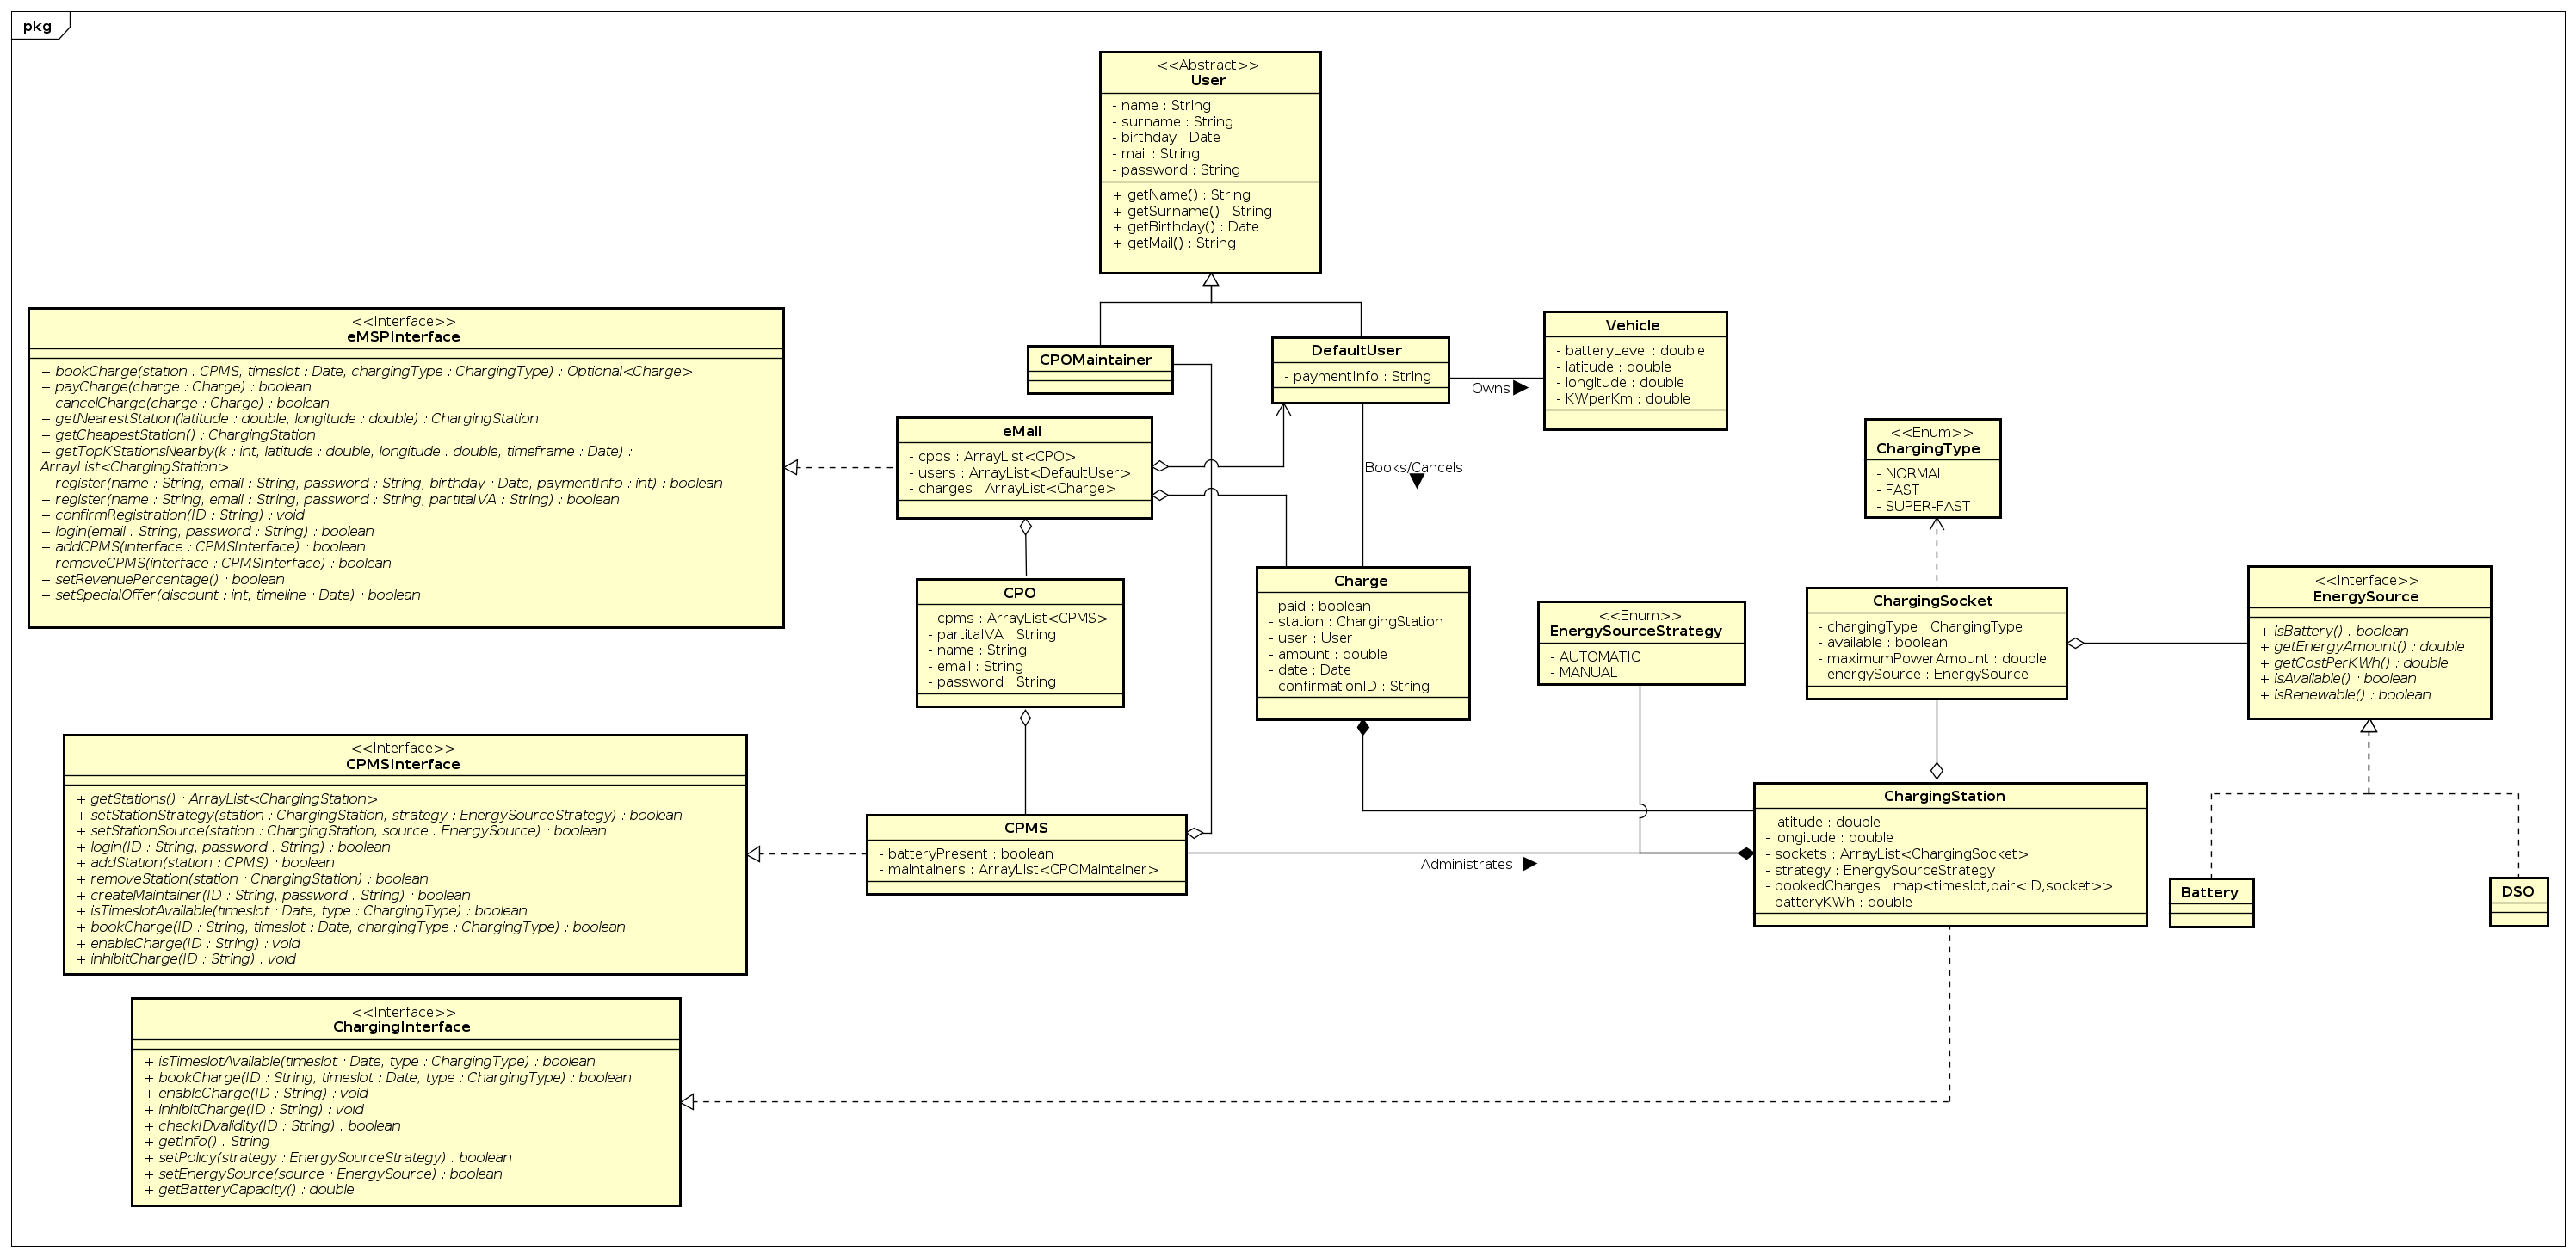
\includegraphics[keepaspectratio, width=16cm]{UML.png}
        \caption{Class diagram}
        \label{fig:UML}
    \end{center}
\end{figure}
In the class diagram illustrated in \autoref{fig:UML} a model (not a functional) view of the system is represented. The \ac{eMall} and \ac{CPMS} interfaces show what the two systems are expected to implement, whereas for the ChargingInterface it is assumed an already existing implementation.
\subsection{Deployment view}
\subsection{Runtime view}
\subsection{Component interfaces}
\subsection{Selected architectural styles and patterns}
\subsection{Other design decisions}
\clearpage